% This is samplepaper.tex, a sample chapter demonstrating the
% LLNCS macro package for Springer Computer Science proceedings;
% Version 2.20 of 2017/10/04
%
\documentclass[runningheads]{llncs}
\usepackage{soul}
\usepackage{tikz}
\usetikzlibrary{calc}
\usepackage{graphicx}
\usepackage{tabularx}




\begin{document}
%
\title{An Event-based Architecture for Cross-Breed Multi-population  Optimization Algorithms}
%
%\titlerunning{Abbreviated paper title}
% If the paper title is too long for the running head, you can set
% an abbreviated paper title here
%
\author{XXXXXXXXXX\inst{1}\orcidID{0000-1111-2222-3333} \and
XXXXXXXXXX\inst{1}\orcidID{1111-2222-3333-4444} \and
XXXXXXXXXX\inst{2}\orcidID{2222--3333-4444-5555}}
%
\authorrunning{XXXXXXXXXX et al.}
% First names are abbreviated in the running head.
% If there are more than two authors, 'et al.' is used.
%
% \institute{National Technological Institute of Mexico
\institute{Hidden institute
\email{XXXXXXXXXX@XXXX.com}\\
%\url{http://www.springer.com/gp/computer-science/lncs}\\
\email{\{abc,lncs\}}}
%
\maketitle              % typeset the header of the contribution
%
\begin{abstract}
  % It seems like the abstract is incompleate, it is a good idea to 
  % write it at the end - Mario
  % You can't present software implementations, but a methodology that
  % you have tested - JJ
  In this work, we present a software implementation that follows an
  event-driven architecture, designed to asynchronously distribute the
  processing of population-based algorithms. The search algorithm uses a
  multi-population approach, creating multiple populations with different
  parameters of execution, allowing the implementation of multiple algorithms, in
  this case Genetic Algorithms (GAs) and Particle Swarm Optimization (PSO).
  Using a message queue, each population is handled by asynchronous
  serverless functions, taking advantage of functional programming
  % "taking advantage of" is not really it. Really, it needs to be
  % that way.
    % \cite{Kunasaikaran2016}
    % No citations in abstract.
    .This cloud-based JavaScript implementation includes a web-based
    application for
    % Why is it cloud ready? - JJ
    the configuration and interaction with algorithms. We executed
    several
    % That's an implementation detail - JJ
    experiments to validate the system, using benchmark functions and
    several configurations. Results show ...

    % Results here 

   % Having
   % the knowledge that both of them are population-based algorithms it can be
   % defined that a migration between 2 or more populations are possible, and
   % this type of hybrid could be helpful to increase the possibility to find the
   % optimal result (the best of the best), there is where fits the concept of
   % Multi-population. 


\keywords{Multi-population  
  \and Asynchronous 
  \and Sub-population 
  \and Serverless 
  \and Distributed.
  \and cross-breed multi-population}
\end{abstract}
%
%
%
\section{Introduction}

In the past few decades, nature-inspired optimization algorithms have been
applied to solve complex real-world problems \cite{yang2014nature}. Algorithms
inspired in natural processes,  include evolutionary algorithms (EAs)
\cite{back1996evolutionary} and swarm intelligence (SI) \cite{kennedy2006swarm}.
These population-based algorithms share the common characteristic of using an initial set of
random candidate solutions that are later used to generate a new set of
candidates, using a nature-inspired heuristic.
%%% Optional
% Maybe to much detail, this list is optional. It is Is here to remind the reader 
% of the plethora of algorithms available; many have been applied successfully to tackle complex problems.  
% if accepted references will be added
Popular EAs are Genetic Algorithms (GAs), Genetic Programming (GP), 
grey wolf optimization (GWO) and Differential Evolution (DE), 
while examples of (SI) are particle swarm optimization (PSO) and
ant colony algorithms (ACO).
%%% 
% Insert here a quick reminder of the island model in GAs 
%   
%%%
%%%
% General definition of multi-population to cover all methods 
% Highlighting the differences 
In general, multi-population based methods divide the original
population into smaller subpopulations or islands, in which each subpopulation
iterates independently. This isolation helps in maintaining an overall diversity
because each subpopulation will search in a particular area. Recombination or
migration between subpopulations is needed to avoid a premature convergence of
candidate solutions. An additional advantage of multi-populations is that each
subpopulation could be processed in parallel. Several works in multi-population
optimization demonstrate that the method can easily
integrate various nature-inspired optimization algorithms, and it often performs
better than single-population optimization algorithms 
\cite{wu2016differential,nseef2016adaptive}.
% Connect with the idea of heterogeneous populations 
% Explan the proposed method of mixing many algorithms through population streams  



%A universe of candidate solutions can exist for a single optimization problem,
%and sometimes conversional algorithms like Genetic Algorithms or Particle Swarm Optimization, 
%for their own are too slow or fail to find an optimal
%solution. As the known No Free Lunch theorem says there is no perfect algorithm 
%that will work for everything and % What do you mean by "traditional" methods? - JJ
% That is why heuristic, population-based algorithms, and other types of
% methods can be applied to find a good enough solution in a reasonable
% time-frame. Population-based algorithms are useful to solve combinatory
% problems; however,  the performance of an algorithm depends on the problem and
% initial conditions. Usually, an algorithm is suitable for only a specific type
% of problems, and it is not always easy to know which algorithm is more
% fitting.
% Up to here this is already known in an evolutionary algorithm
% conference. I also don't get your point
% Probably what you want to say is something along the lines of
% "The no free lunch theorem states that there's no single algorithm
% that can find adequate solutions for all possible problems. In
% general, a single algorithm will need fine-tuning of its parameters
% to find the best possible solution in an adequate amount of
% time...."
% Then you can continue into the next paragraph, where you propose a
% solution - JJ
%% 
even assuming that we selected an appropriate algorithm, we must also find the
appropriate parameters.  Some parameters affect the accuracy of the solution and
the convergence speed of the algorithms as they affect the degree of exploration
or exploitation of the search space.  cross-breed multi-population algorithm that combine two or more
heuristics can benefit from the strengths of each. % You need to
                                % define what you mean by hybrid
                                % algorithm. Actually, this algorithms
                                % is not hybrid, but a combination of
                                % several algorithms. - JJ 

For instance, a genetic
algorithm could find a promising global solution that is not optimal while another algorithm, more
suitable for a local search, finds the global optimum. To deal with these problems,
parallel and cross-breed multi-population algorithms architecture have been proposed. % Parallel
                                % architectures were proposed mainly
                                % for speed. You really need to
                                % qualify this - JJ
The clear advantage of
these architectures is the faster execution of the algorithms. However, there is
also the ability to change the search dynamically, % You can do that
                                % in sequential architectures too - JJ
having multiple algorithms
with different parameters interacting with each other at the same
time. % Now you're arriving somewhere. But you need to:
% 1. Add more references. Most claims must have a reference to support it.
% 2. State clearly from the beginning, and in a positive way (that is,
% don't use the reasoning: this sucks, so we need something better)
% what is your intention: use a parallel architecture for combined,
% parameter-free-algorithms.
% 3. 

In this work, we present an implementation of an event-driven architecture
proposed in [Anonymous]; this is a so-called {\em serverless}
architecture that
processes independent small populations with their own characteristics % small? fragments? Aren't they independent populations?
from a population of populations in a distributed way, working together to find an optimal value. % they're simply independent
                                % populations - JJ
The main components are stateless functions,
running asynchronously, and communicating using message-queues, that process each
sub-population. Also, sub-populations use the migration of data between them, to
help each other even if the algorithms or parameters of each sub-population are
different. The objective is to prevent the algorithm from falling into optimal
local values balancing inconvenients of a determinated population-based algorithm with the others.
This mechanism is driven by events, on arriving processed sub-population migrating with a random selection 
from the best 2 sub-populations, keeping diversity but with a sort of elitism. 
% But simple parallel evolutionary algorithms can also do the same
% thing. You don't need to use two algorithms at the same time - JJ
% This new
% implementation uses JavaScript for the full stack, and it is designed to be
% executed locally or in a cloud environment. The implementation includes a
% web-based application to execute and monitor experiments
% interactively. % implementation detail, best left for the conclusions
               % - JJ
We also
propose alternative methods of migration between populations to compensate for
differences in the execution time of the functions. % This is probably
                                % one of the main points of the
                                % paper. Should be enphasized more
                                % - JJ


%This document shows what are serverless functions and their spot into the world
%of software architecture, describing its features and advantages of its
%implementation compared with others. Once that the concept of Serverless is
%understood  
% I think this can be explained briefly in the state of the art - Mario

%%%%% BEGIN (needs work)

To evaluate the software implementation and the capability of a cross-breed multi-population solution,
we conducted several experiments using different benchmark functions, comparing the
results of single versus cross-breed multi-population algorithms. For the experiments, we choose to
compare the PSO and GA algorithms, as they are well understood, and there are
several implementations in the literature. We implemented both algorithms as
stateless functions, and more algorithms can be added in the same way.

%%%%% END (needs work): - Mario

%%
%% A description of the paper goes here
%% what are we proposing? You can start with the description in the abstract.  
%% what are the findings? 
%% what is presented in each section? 
%% Check other papers to get the idea - Mario

The rest of the paper is organized as follows: next section is devoted
to analyzing the state of the art in multi-population, multi-paradigm,
stateless evolutionary algorithms. The architecture proposed is
presented in Section \ref{sec:architecture} and put to work in the
Section \ref{sec:exp}. Finally, we present our conclusions and the
future lines of work.

\section{State of the Art}

% The title of these subsections will be removed, they are just place-holders
% References are pending
\subsection{Multi-population}

% Connect with the idea of heterogeneous populations 
% Mixing many algorithms   




\subsection{Parallel, Distributed}
Multi-population algorithm are initial



Distributed and cloud-based architectures are used extensively in the software
industry because of their high performance and lower overall cost. Many systems
are being created and migrating step by step to microservices and new serverless
architectures, which proposes the use of Function as a Service (FaaS) 
\cite{Hellerstein2018,Everywhere,Baird2016}. 
Researchers are starting to exploit this type of architectures in heuristic optimization
development, and here we take advantage of them to increase the performance of
some population-based algorithms.

\subsection{Cloud, Serverless}
% These sections can be optional, 
% they can be part of the Intro, SoA, of a Concepts section - Mario

% Multi-population
% Parallel, Distributed 
% Cloud
% Serverless

Recently, cloud providers such as Amazon Web Services (AWS), IBM Cloud, and
Google Cloud, offers a new alternative to programming through interfaces called
Serverless Computing [References], this platform consists of an effortless a
mechanism where developers upload the code into the platform and execute it as
many times as it is required, scaling and allowing to do this in parallel. This
way, the developers do not worry about servers, connections, and other
configurations. In serverless, users pay only for what it is used. There is also
the option to install some of these platforms locally; for instance, AWS (Amazon
Web Services) \cite{Baird2016} or Apache Open Whisk \cite{Guerv2018}. 


\begin{figure}[htp]
  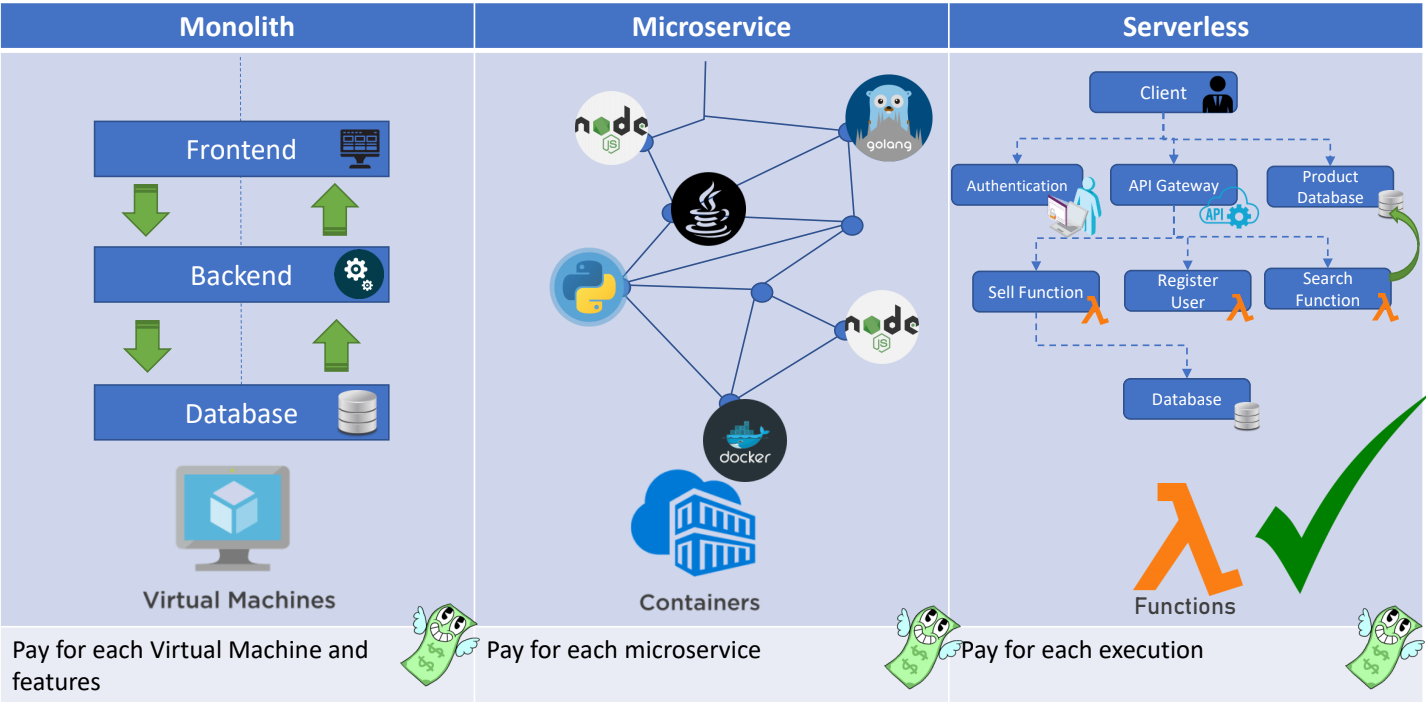
\includegraphics[width=\textwidth]{img/architectures.png}
  \caption{Software architecture generations.} \label{fig1}
  \end{figure}

\subsubsection{Serverless Function} 
In math, a function is a relation between a set of inputs and an allowed set of
outputs, with the idea that each input goes to a single output. However, in
computer science, a function is defined as a unit of code that has a role in a
greater code structure, works on various inputs that usually are variables and
throws a concrete output that is the result of the process those variables. One
of the main features that belong to functions is that they are stateless, they
are focused on inputs and result with a simple process that does not require a
state, at the moment the inputs get into the function are already generating an
output. In serverless, events such as messages or HTTP requests can trigger
these functions. Also, each function scales independently and is stateless with
a short duration \cite{Baird2016,Cook2017}.
% I am not a fan of that definition of a function in CS - Mario
% Explain a bit more the "Stateless" part - Mario 

\subsection{Asynchronous}

Asynchronous algorithms consist of performing a certain action such as the
movement of the particles in PSO or the crosses and mutations of the GA without
the need for the execution of one to affect the other, in a few words a
Individual execution of each without waiting times. This is very useful. when
several threads are used in parallel execution because if the expected response
of action, for example, a GA of 100 generations and a GA of 10 is it is
preferable not to stop the search and give priority to 10 generations
\cite{Santander-jim2018,Sherry2012,Goebel2016,Guerv2018}. Asynchronous functions
are created in programming that has promising results response that is immediate
and does not stop the main execution by secundary actions
\cite{Moroney2017,Ambler2015}.

An asynchronous architecture has what is known as execution queues in the that
can be appreciated that give an added value that gives advantage over other
architectures by reducing waiting times and neglecting the concept that order is
important, of course, this type of architectures is not applicable to all cases
but speaking in distributed systems where multiple population-based algorithms
are executed with parallel execution, they result in a better degree of
efficiency, in addition to reducing the number of control parameters since they
require having a decoupled architecture \cite{Ma2019,Santander-jim2018}.

\subsection{Functional Programming}

It is a very important programming paradigm that is based on lambda expression,
created from math knowledge. The programming languages could be classified by
programming styles, there are usually known as programming paradigms
\cite{Kunasaikaran2016}.

In the functional programming style the data does not exist independently or by
themselves, but these happen in the form of arguments and are transformed as a
flow in an exit through the functions. Each function is described as atomic
because each one only has a simple operation that generates an expected result
\cite{Kunasaikaran2016}.


\section{Proposed architecture}
\label{sec:architecture}

The proposal is an architecture that allows processing of a single population
that is divided into sub-populations, distributing them to processes in different
ways, and then communicating with each other with the purpose of increasing the
possibility to find the highest fitness of a function. This architecture can accept
the use of an indeterminate number of algorithms, allowing an easy cross-breed multi-population 
and continuous adaptability for different problems. % A reference to a
                                % figure should go around here - JJ

% Before nodes, you need to explain the overall layout of the
% architecture - JJ
This architecture consist in 3 nodes, % Nodes or types of nodes?
they are explained on the next points:

\begin{itemize}
  \item {\bf Manager}: This node creates a population conformed by sub-populations is created and the architecture
  initialize parameters to run the algorithm. Every time a sub-population is
  created triggers an event that sends the subpopulations to be stored in a 
  JSON file into the MongoDB data store (preventing to saturate the
  memory) % what do you mean here? - JJ
  and to a message queue
  that is directed to its subsequent processing in the “Receiver” section that
  is our cluster of functions (Faas), because each sub-population requires the
  execution of a different algorithm, there is a different channel in the web
  sockets for each type of algorithm that triggers its respective serverless
  function. Once a subpopulation is processed, it is returned and a selection is
  made for the sub-population migration. The migration selection is made by
  taking the population attribute of the subpopulation that was returned and the
  subpopulation that it has been selected among the best 2, it should be noted
  that the decision to identify the best from the 2 is made randomly. Once the
  selection is made, a Splitting Point Uniform crossing will be made. The 2 new
  subpopulations replace their self and are resent it back to their respective
  serverless function and this process is repeated until completing the number
  of assigned migrations for the multi-population
  \cite{Ma2019,Santander-jim2018}. Of course this whole process is performed
  asynchronously avoiding the wait for all responses from serverless functions
  to perform a crossover or an update of the multi-population status
  \cite{Lovbjerg2001,Jimeno2019}. In the following figure, you can see from the
  illustrative way how the multi-population is composed.
% \begin{figure}[htp]
%   \centering
%   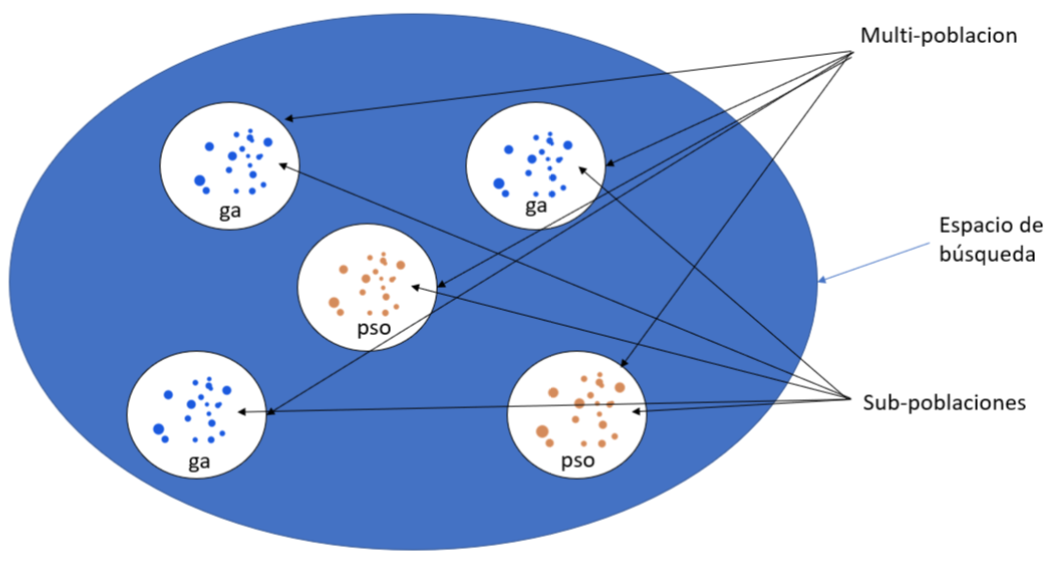
\includegraphics[width=0.7\textwidth]{img/multipopulation.png}
%   \caption{Multipopulation representation.} \label{fig1} %This is defined twice. 
%   \end{figure}
  The mechanism to send the sub-population to the serverless functions is
 creating a queue with a dimension of 2 positions that asynchronously allow
 communicating.
\item {\bf Message Provider}: Its purpose is the creation of a sub-population messages
  queue which is the communication channel % A queue is not a channel,
                                % it's _in_ a channel - JJ
  between the sub-population Manager and
the Receiver (FaaS), each message is a trigger for the execution of a GA or PSO
function. Thanks to the message queue, it is possible to perform the serverless
functions asynchronously, avoiding waiting states in the algorithm
while responses arrive, 
independently of their duration and the simultaneous evaluation of different
sub-populations independent of its algorithm or characteristics.
\item Receiver: The following section contains the Serverless
  functions of the % which section? Are you talking about the receiver
                   % itself? - JJ
algorithms to be executed, reducing the best possible using the functional
programming paradigm so that they can be converted into FaaS without problems,
in addition to achieving a completely clean and fast
execution\cite{Roberts2016}. Each message received on this node is executed in
the form of a multi-threaded process in parallel, this allows having more than
one population-based search algorithm running at the same time and making a copy
of itself each algorithm functions as required.
\end{itemize}

To develop this architecture the applied technologies are based in JavaScript
using Node JS as it can be seen in the General Architecture Flowchart
shown in Figure \ref{fig2}.

% I don't think this figure is appropriate for a paper.
\begin{figure}[htp]
  \centering
  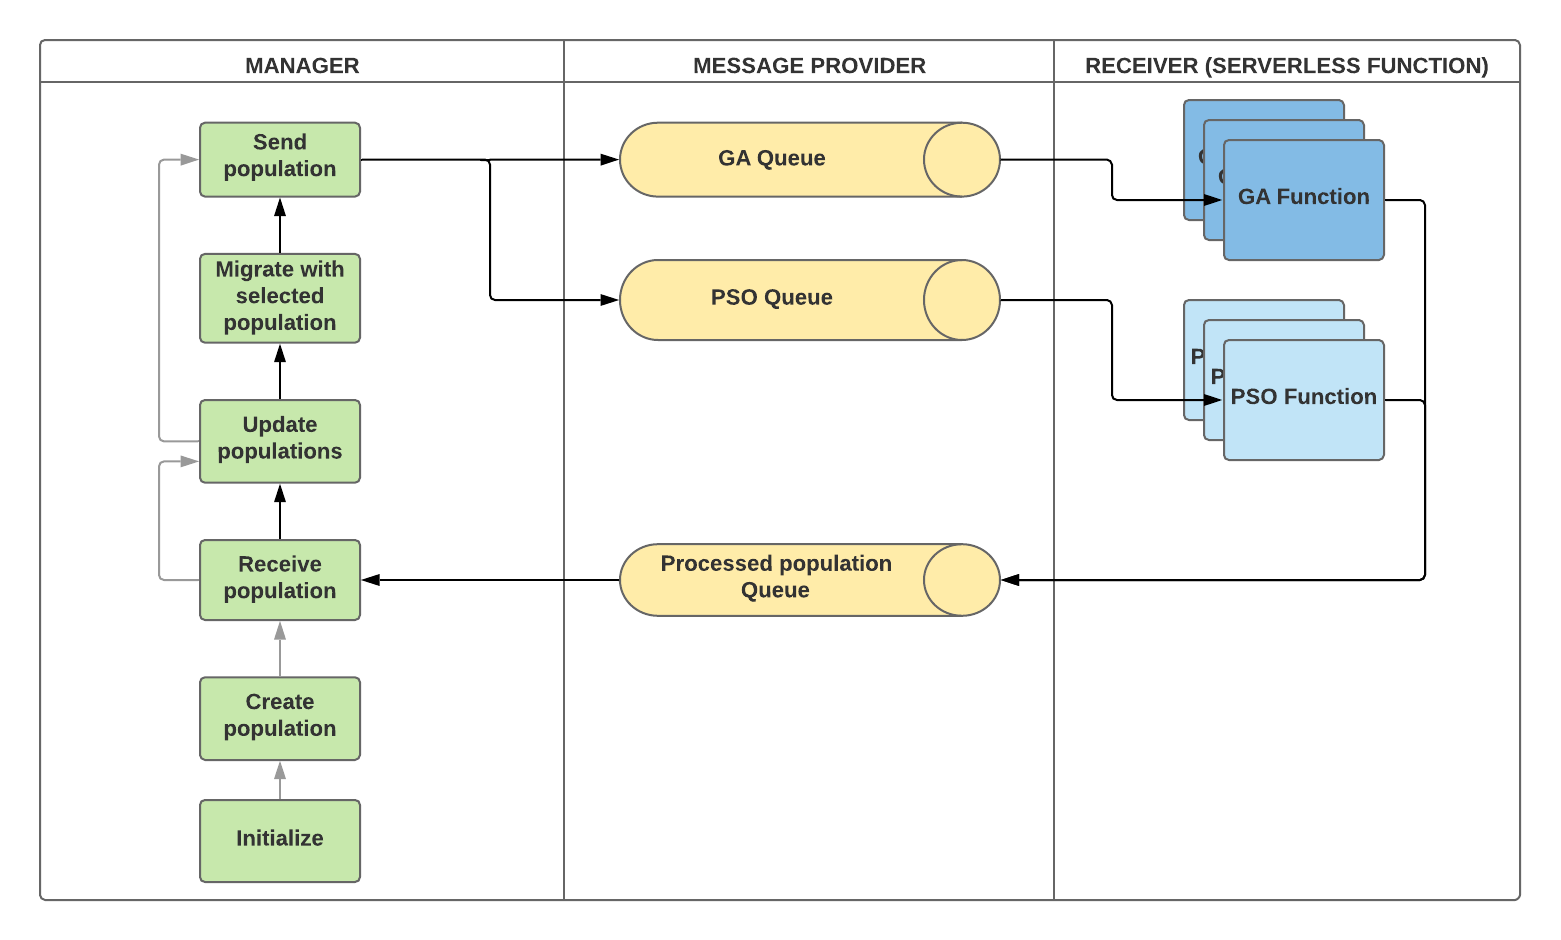
\includegraphics[width=0.9\textwidth]{img/Architecture diagram.png}
  \caption{General Architecture Flowchart.} \label{fig2}
  \end{figure}
  % Could be OK for the presentation, divided in 3 slides - JJ
  
\subsection{Sub-population definition}

Individuals are created composed of 2 types of information, the one that is
active or useful for crossing and the one that is not. % this is not a
                                % proper definition. - JJ
The population contains
the series of possible solutions, while the rest % what is the rest? -
% JJ
% Please rewrite this - JJ
contains the information on how
the processing for the search of the optimal solutions will be executed, linked
directly with their respective algorithms.
Y
\begin{figure}[htp]
  \centering
  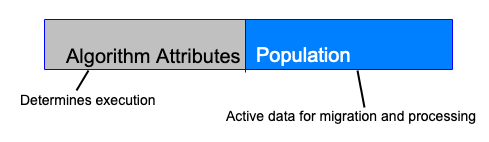
\includegraphics[width=0.6\textwidth]{img/subpopulationDefinition.png}
  \caption{Sub-population composition.} \label{fig3}
  \end{figure}

\subsection{Splitting Point Uniform Migration}

This architecture communicates sub-populations using migrations,
taking
% It's not an architecture, unless you mean the overall architecture - JJ
information from 2 sub-populations and mixing them using a process similar to a
crossover in Genetic Algorithms, creating 2 completely new sub-populations every
time a processed sub-population arrives into the Manager node and replacing
themselves in the multi-population.

The migration created to % to? For? - JJ
this architecture is a method called Splitting Point
Uniform that consists of a uniform mask that is created to apply the migration
between individuals, vectors or both of them, from two sub-populations. The
selected data are combined using the midpoint between the active values
points by the binary mask generated randomly. % Not clear. Maybe a
                                % picture? - JJ
This process iterates the 2
sub-populations to randomly swap values and replaces some of them with middle
points \cite{Kramer2017,Kaya2011}.


\begin{figure}[htp]
  \centering
  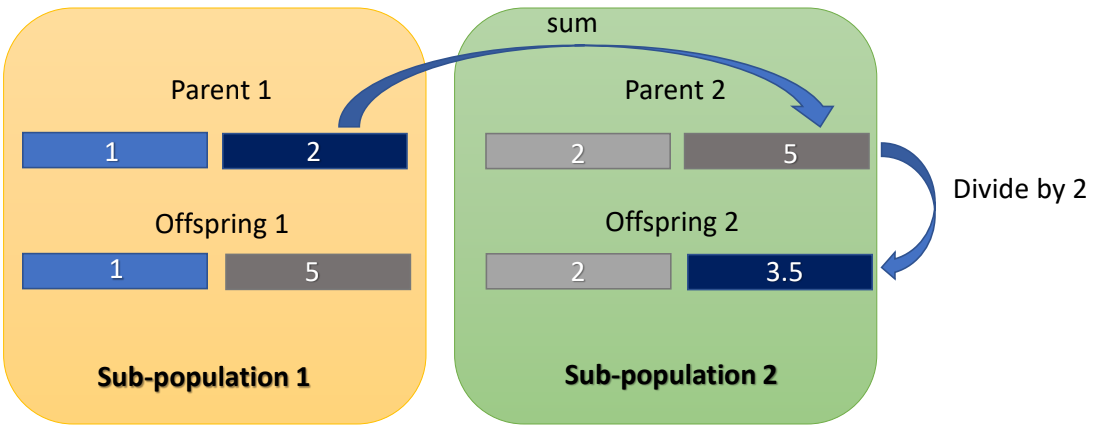
\includegraphics[width=0.9\textwidth]{img/splittinPointUniform.png}
  \caption{Splitting Point Uniform process.} \label{fig4}
  \end{figure}

  \subsection{Migration Selection} The 2 sub-populations selected to realize
  migration is one arrived sub-population from a serverless function and another
  one using selection by tournament keeping up the information of the best
  sub-population of the multi-population but without discarding possible
  sub-populations that in a near future could be the clue to find optimal
  values.

\begin{figure}[htp]
  \centering
  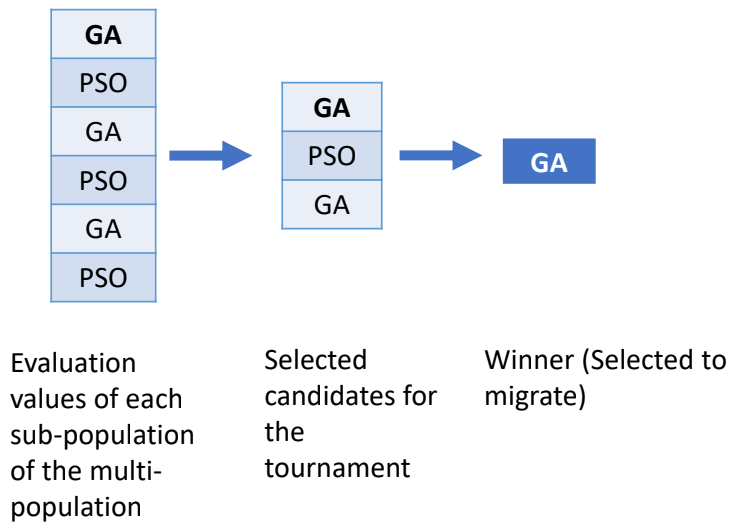
\includegraphics[width=0.5\textwidth]{img/selection.png}
  \caption{Selection by tournament.} \label{fig5}
  \end{figure}


  \section{Experiments and Results}
  \label{sec:exp}
  
\subsection{Experiments}
Now that interaction between sub-populations with different algorithms is
working and cross-breed multi-population has been a success, using until now the added
algorithms (GA and PSO) algorithms \cite{Kramer2017,Guerrero2017,Lalwani2019},
all thanks to the developed architecture, let's proceed to the experiments. This
section is going to be the execution of several experiments from 2 to 40
dimensions, with a stop criteria of an error below 0.5E-8, without a parameter
optimization method, waiting that the architecture by itself would be enough
to increase the possibility of finding a better optimal result than the traditional
methods. All this hoping that the results will probe % probe or prove?
                                % - JJ
the needs of this kind of
architecture on increasing dimensions. To test if the architecture was useful,
several experiments were made to solve benchmark functions, for this case the
functions are Sphere, Rastrigin and Rosenbrock. Using 10 sub-population for each
experiment and a maximum of 4 migrations per sub-population with different
algorithms and parameters for each sub-population.

\begin{figure}[htp]
  \centering
    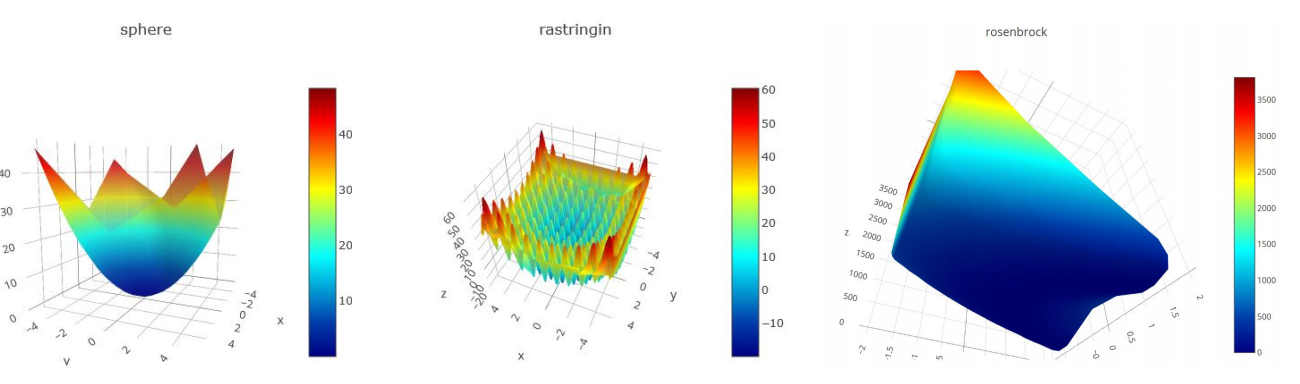
\includegraphics[width=0.7\textwidth]{img/benchmark.png}
    \caption{Benchmark functions for experimentation.} \label{fig6}
    \end{figure}

\subsection{Parameter Configuration} 

This architecture modifies the traditional way of working with population-based
algorithms, then the experiments could not be parameterized as they
usually are. % Probably rewrite this sentence - JJ

Then the experiments are scaled by their number of evaluations and the
parameters must be configured to be adjusted to the next criteria, using the
next expression: % I don't understand this sentence - JJ

\begin{equation}
    \label{eq:hesitancy-interpretation}
   Evaluations = 10^{5} Dimensions
   \end{equation}

   For example, if the experiment has 2 dimensions, the maximum number of
   evaluations will be 200,0000, for 10 dimensions will be 1,000,000 of evaluations
   and the same with the other dimensions.





% How are these parameters computed? - JJ



   \begin{table}[h!tp]
    \caption{Parameters used by the algorithms for 2 and 10 dimensions. The Random mutation for GA includes the Tournament2, Tournament3, Random, RandomLinearRank, Sequential, Fittest variants. Fitness function is minimized in both cases.}
    \label{table:ga-pso-parameters-2}
    \centering
    \begin{tabularx}{\linewidth}{|l|X|X|X|X|}
    \hline
    Parameter & \multicolumn{4}{c|}{Values for dimensions} \\
      \hline
      & 2 & 10 & 20 & 40 \\
    \hline
    GA Generations & 50 &  \multicolumn{3}{c|}{70} \\
    \hline
     GA Population size & 100 &  \multicolumn{3}{c|}{200}\\
    \hline
    GA Mutation &  \multicolumn{4}{c|}{Random}\\
    \hline
    GA Crossover selection & \multicolumn{4}{c|}{Tournament3} \\
    \hline
    GA Crossover percentage & \multicolumn{4}{c|}{Random[10\%, 80\%]} \\
    \hline
    GA Mutation percentage & \multicolumn{4}{c|}{Random[10\%,50\%]} \\
    \hline
    GA Crossover function & \multicolumn{4}{c|}{1 point crossover} \\
    \hline
    GA Mutation Function & \multicolumn{4}{c|}{Gaussian} \\
      \hline 
      \hline
    PSO Iterations & 50 & \multicolumn{3}{c|}{70} \\
    \hline
    PSO Vector size & 100 & \multicolumn{3}{c|}{200} \\
    \hline
    PSO Social factor & \multicolumn{4}{c|}{Random[0.5,4.0]} \\
    \hline
    PSO Individual factor & \multicolumn{4}{c|}{Random[0.5,4.0]} \\
    \hline
    PSO Inercia factor & \multicolumn{4}{c|}{Random[0.5,4.0]} \\
    \hline
    \end{tabularx}
    \end{table}

% \begin{figure}[htp]
% 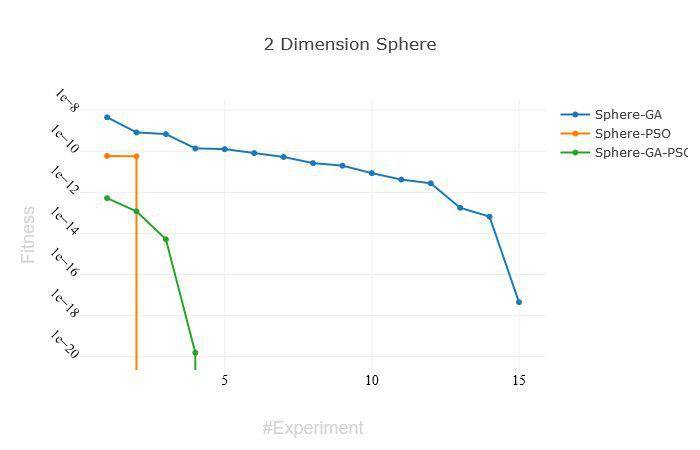
\includegraphics[width=\textwidth]{img/2-sphere.jpg}
% \caption{2 dimension experiments Sphere.} \label{fig7}
% \end{figure}

% \begin{figure}[htp]
%   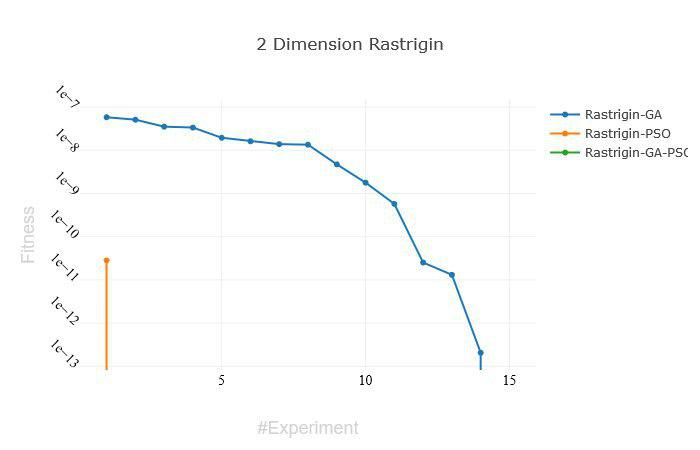
\includegraphics[width=\textwidth]{img/2-rastrigin.jpg}
%   \caption{2 dimension experiments Rastrigin.} \label{fig8}
%   \end{figure}
  
% \begin{figure}[htp]
%   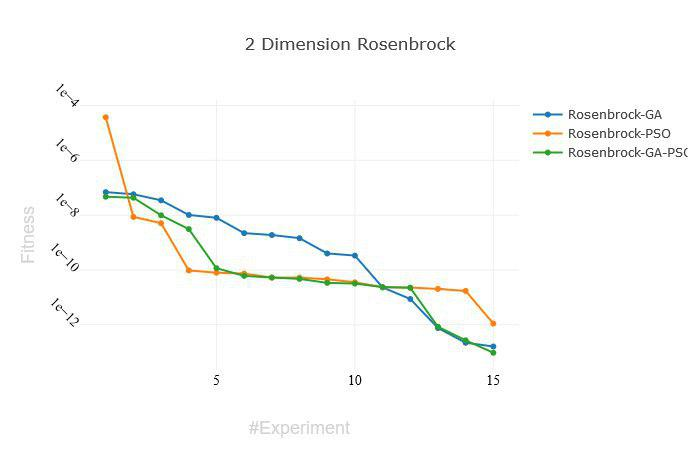
\includegraphics[width=\textwidth]{img/2-rosenbrock.jpg}
%   \caption{2 dimension experiments Rosenbrock.} \label{fig9}
%   \end{figure}

\begin{table}[htp]
    \caption{2 dimensional experiment results}
    \label{table:resultados-2}
    \centering
    \begin{tabular}{|c|c|c|c|}
    \hline
    Fn & Best & AVG & Experiment Number \\
    \hline
    \hline
    Rastrigin GA & 0 & 1.65377E-08 & 15\\
    \hline
    Rastrigin PSO & 0 & 1.8872E-12 & 15\\
    \hline
    Rastrigin GA-PSO & 0 & 0 & 15\\
    \hline
    Sphere GA & 4.53222E-18 & 4.36977E-10 & 15\\
    \hline
    Sphere PSO & 0 & 7.8012E-12 & 15\\
    \hline
    Sphere GA-PSO & 0 & 4.33161E-14 & 15\\
    \hline
    Rosenbrock GA & 1.62335E-13 & 1.24176E-08 & 15\\
    \hline
    Rosenbrock PSO & 1.11674E-12 & 2.47795E-06 & 15\\
    \hline
    Rosenbrock GA-PSO & 9.5809E-14 & 6.90695E-09 & 15\\
    \hline
    \end{tabular}
    \end{table}
  

    
      % \begin{figure}[htp]
      %   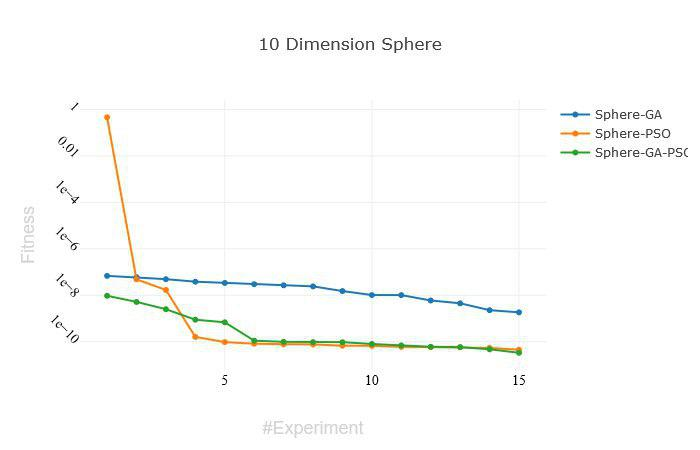
\includegraphics[width=\textwidth]{img/10-sphere.jpg}
      %   \caption{10 dimensions experiments Sphere.} \label{fig10}
      %   \end{figure}

      %   \begin{figure}[htp]
      %     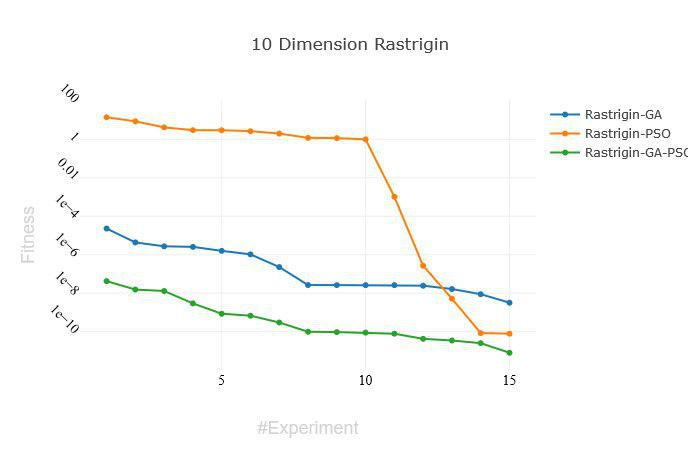
\includegraphics[width=\textwidth]{img/10-rastrigin.jpg}
      %     \caption{10 dimensions experiments Rastrigin.} \label{fig11}
      %     \end{figure}

      %     \begin{figure}[htp]
      %       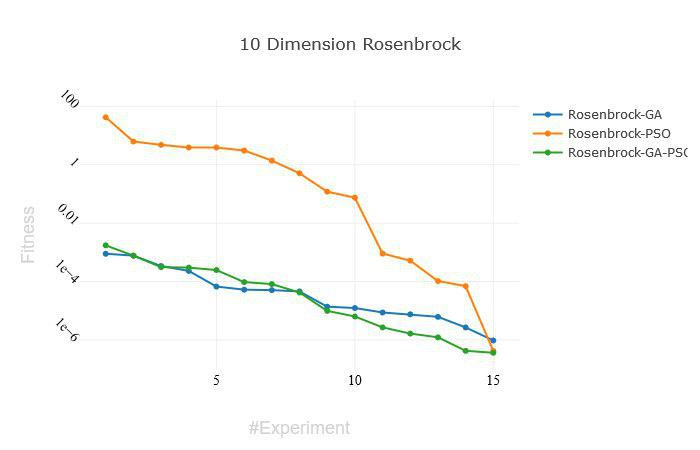
\includegraphics[width=\textwidth]{img/10-rosenbrock.jpg}
      %       \caption{10 dimensions experiments Rosenbrock.} \label{fig12}
      %       \end{figure}

        \begin{table}[htp]
          \caption{10 dimensional experiment results}
          \label{table:resultados-2}
          \centering
          \begin{tabular}{|l|l|l|l|}
          \hline
          Fn & Best & Average & Experiment Number \\
          \hline
          \hline
          Rastrigin GA & 3.21768E-09 & 2.38015E-06 & 15\\
          \hline
          Rastrigin PSO & 7.8586E-11 & 2.715716161 & 15\\
          \hline
          Rastrigin GA-PSO & 8.01492E-12 & 5.08668E-09 & 15\\
          \hline
          Sphere GA & 1.84051E-09 & 2.5389E-08 & 15\\
          \hline
          Sphere PSO & 4.50351E-11 & 4.72855E-09 & 15\\
          \hline
          Sphere GA-PSO & 3.33851E-11 & 1.30062E-09 & 15\\
          \hline
          Rosenbrock GA & 9.58323E-07 & 1.24176E-08 & 15\\
          \hline
          Rosenbrock PSO & 4.16711E-07 & 4.431565444 & 15\\
          \hline
          Rosenbrock GA-PSO & 3.62472E-07 & 0.000240251 & 15\\
          \hline
          \end{tabular}
          \end{table}
          
            % \begin{figure}[htp]
            %   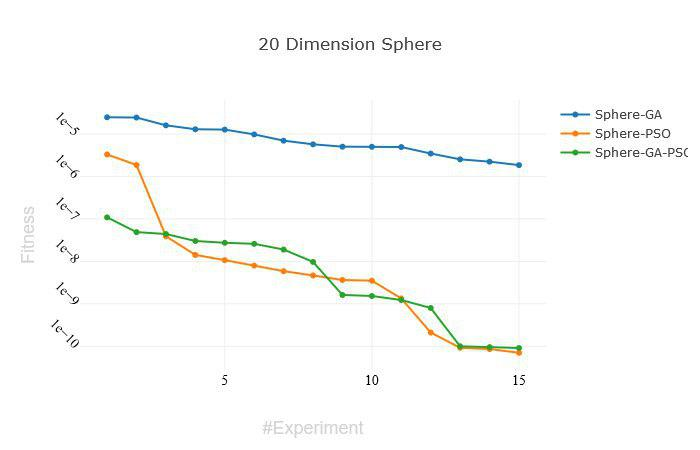
\includegraphics[width=\textwidth]{img/20-sphere.jpg}
            %   \caption{20 dimensions experiments Sphere.} \label{fig13}
            %   \end{figure}
      
            %   \begin{figure}[htp]
            %     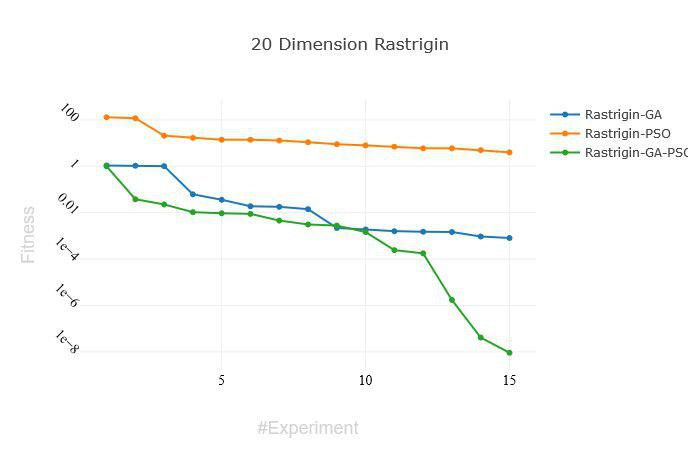
\includegraphics[width=\textwidth]{img/20-rastrigin.jpg}
            %     \caption{20 dimensions experiments Rastrigin.} \label{fig14}
            %     \end{figure}
      
            %     \begin{figure}[htp]
            %       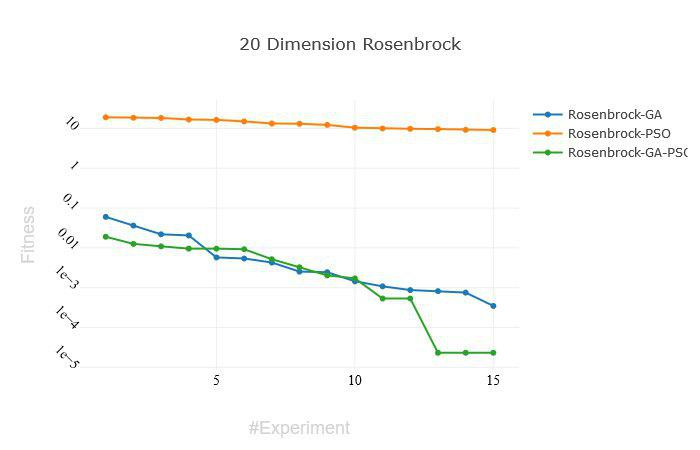
\includegraphics[width=\textwidth]{img/20-rosenbrock.jpg}
            %       \caption{20 dimensions experiments Rosenbrock.} \label{fig15}
            %       \end{figure}

                  \begin{table}[htp]

    \caption{Resultados 20 dimensiones}
    \label{table:resultados-2}
    \centering
    \begin{tabular}{|l|l|l|l|}
    \hline
    Fn & Best & Average & Experiment Number \\
    \hline
    \hline
    Rastrigin GA & 0.000808633 & 0.220596203 & 15\\
    \hline
    Rastrigin PSO & 3.988070734 & 25.51777514 & 15\\
    \hline
    Rastrigin GA-PSO & 9.13E-09 & 7.38E-02 & 15\\
    \hline
    Sphere GA & 1.84051E-09 & 9.22715E-06 & 15\\
    \hline
    Sphere PSO & 7.04E-11 & 3.50E-07 & 15\\
    \hline
    Sphere GA-PSO & 9.11E-11 & 2.13E-08 & 15\\
    \hline
    Rosenbrock GA & 0.000348015 & 0.010958941 & 15\\
    \hline
    Rosenbrock PSO & 9.119539342 & 13.37613983 & 15\\
    \hline
    Rosenbrock GA-PSO & 2.31663E-05 & 0.005608855 & 15\\
    \hline
    \end{tabular}
    \end{table}
    
      % \begin{figure}[htp]
      %   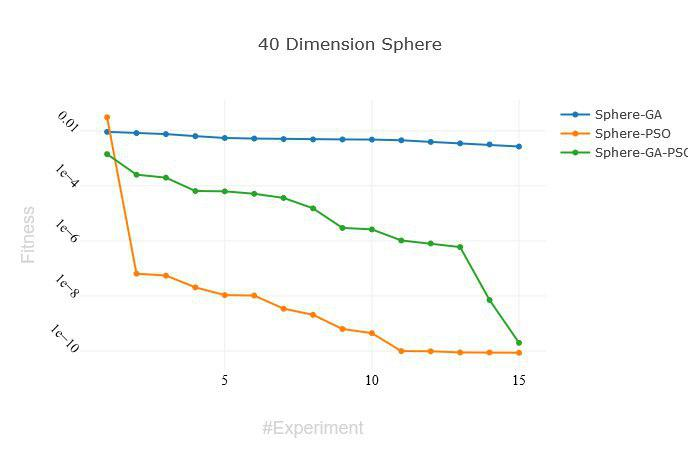
\includegraphics[width=\textwidth]{img/40-sphere.jpg}
      %   \caption{40 dimensions experiments Sphere.} \label{fig1}
      %   \end{figure}

      %   \begin{figure}[htp]
      %     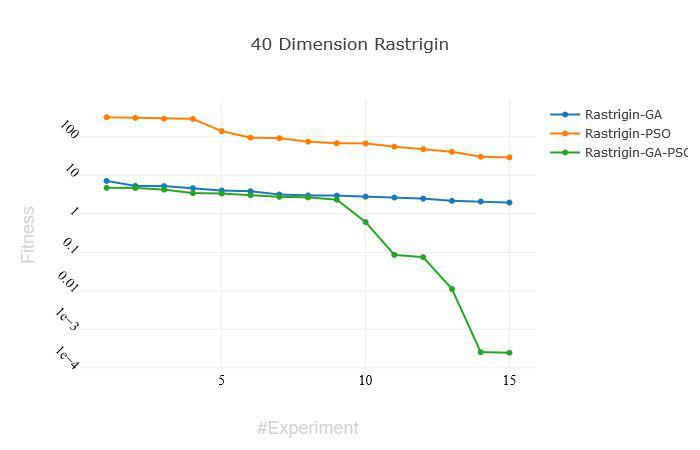
\includegraphics[width=\textwidth]{img/40-rastrigin.jpg}
      %     \caption{40 dimensions experiments Rastrigin.} \label{fig1}
      %     \end{figure}

      %     \begin{figure}[htp]
      %       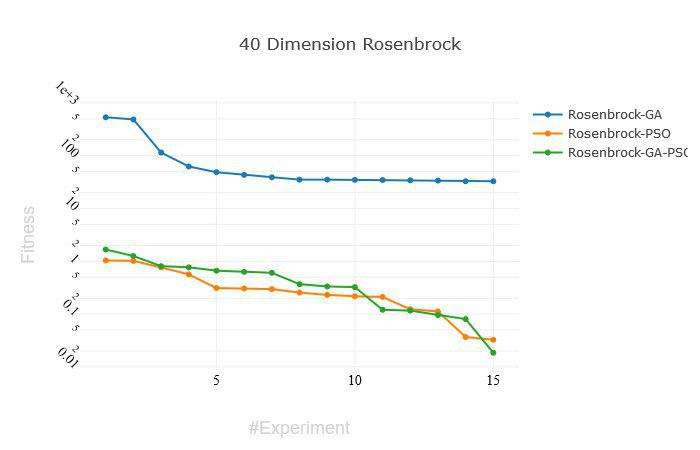
\includegraphics[width=\textwidth]{img/40-rosenbrock.jpg}
      %       \caption{40 dimensions experiments Rosenbrock.} \label{fig1}
      %       \end{figure}

            \begin{table}[htp]
              \caption{Resultados 40 dimensiones}
              \label{table:resultados-2}
              \centering
              \begin{tabular}{|l|l|l|l|}
              \hline
              Fn & Best & Average & Experiment Number \\
              \hline
              \hline
              Rastrigin GA & 1.95478879 & 3.560837088 & 15\\
              \hline
              Rastrigin PSO & 29.06596132 & 130.2865863 & 15\\
              \hline
              Rastrigin GA-PSO & 2.46E-04 & 2.13E+00 & 15\\
              \hline
              Sphere GA & 0.002686956 & 0.005302951 & 15\\
              \hline
              Sphere PSO & 8.68E-11 & 2.07E-03 & 15\\
              \hline
              Sphere GA-PSO & 2.00E-10 & 1.41E-04 & 15\\
              \hline
              Rosenbrock GA & 0.000348015 & 106.9287542 & 15\\
              \hline
              Rosenbrock PSO & 0.032708559 & 0.368395353 & 15\\
              \hline
              Rosenbrock GA-PSO & 0.018538924 & 0.525086565 & 15\\
              \hline
              \end{tabular}
            \end{table}

            \begin{figure}
              \centering
                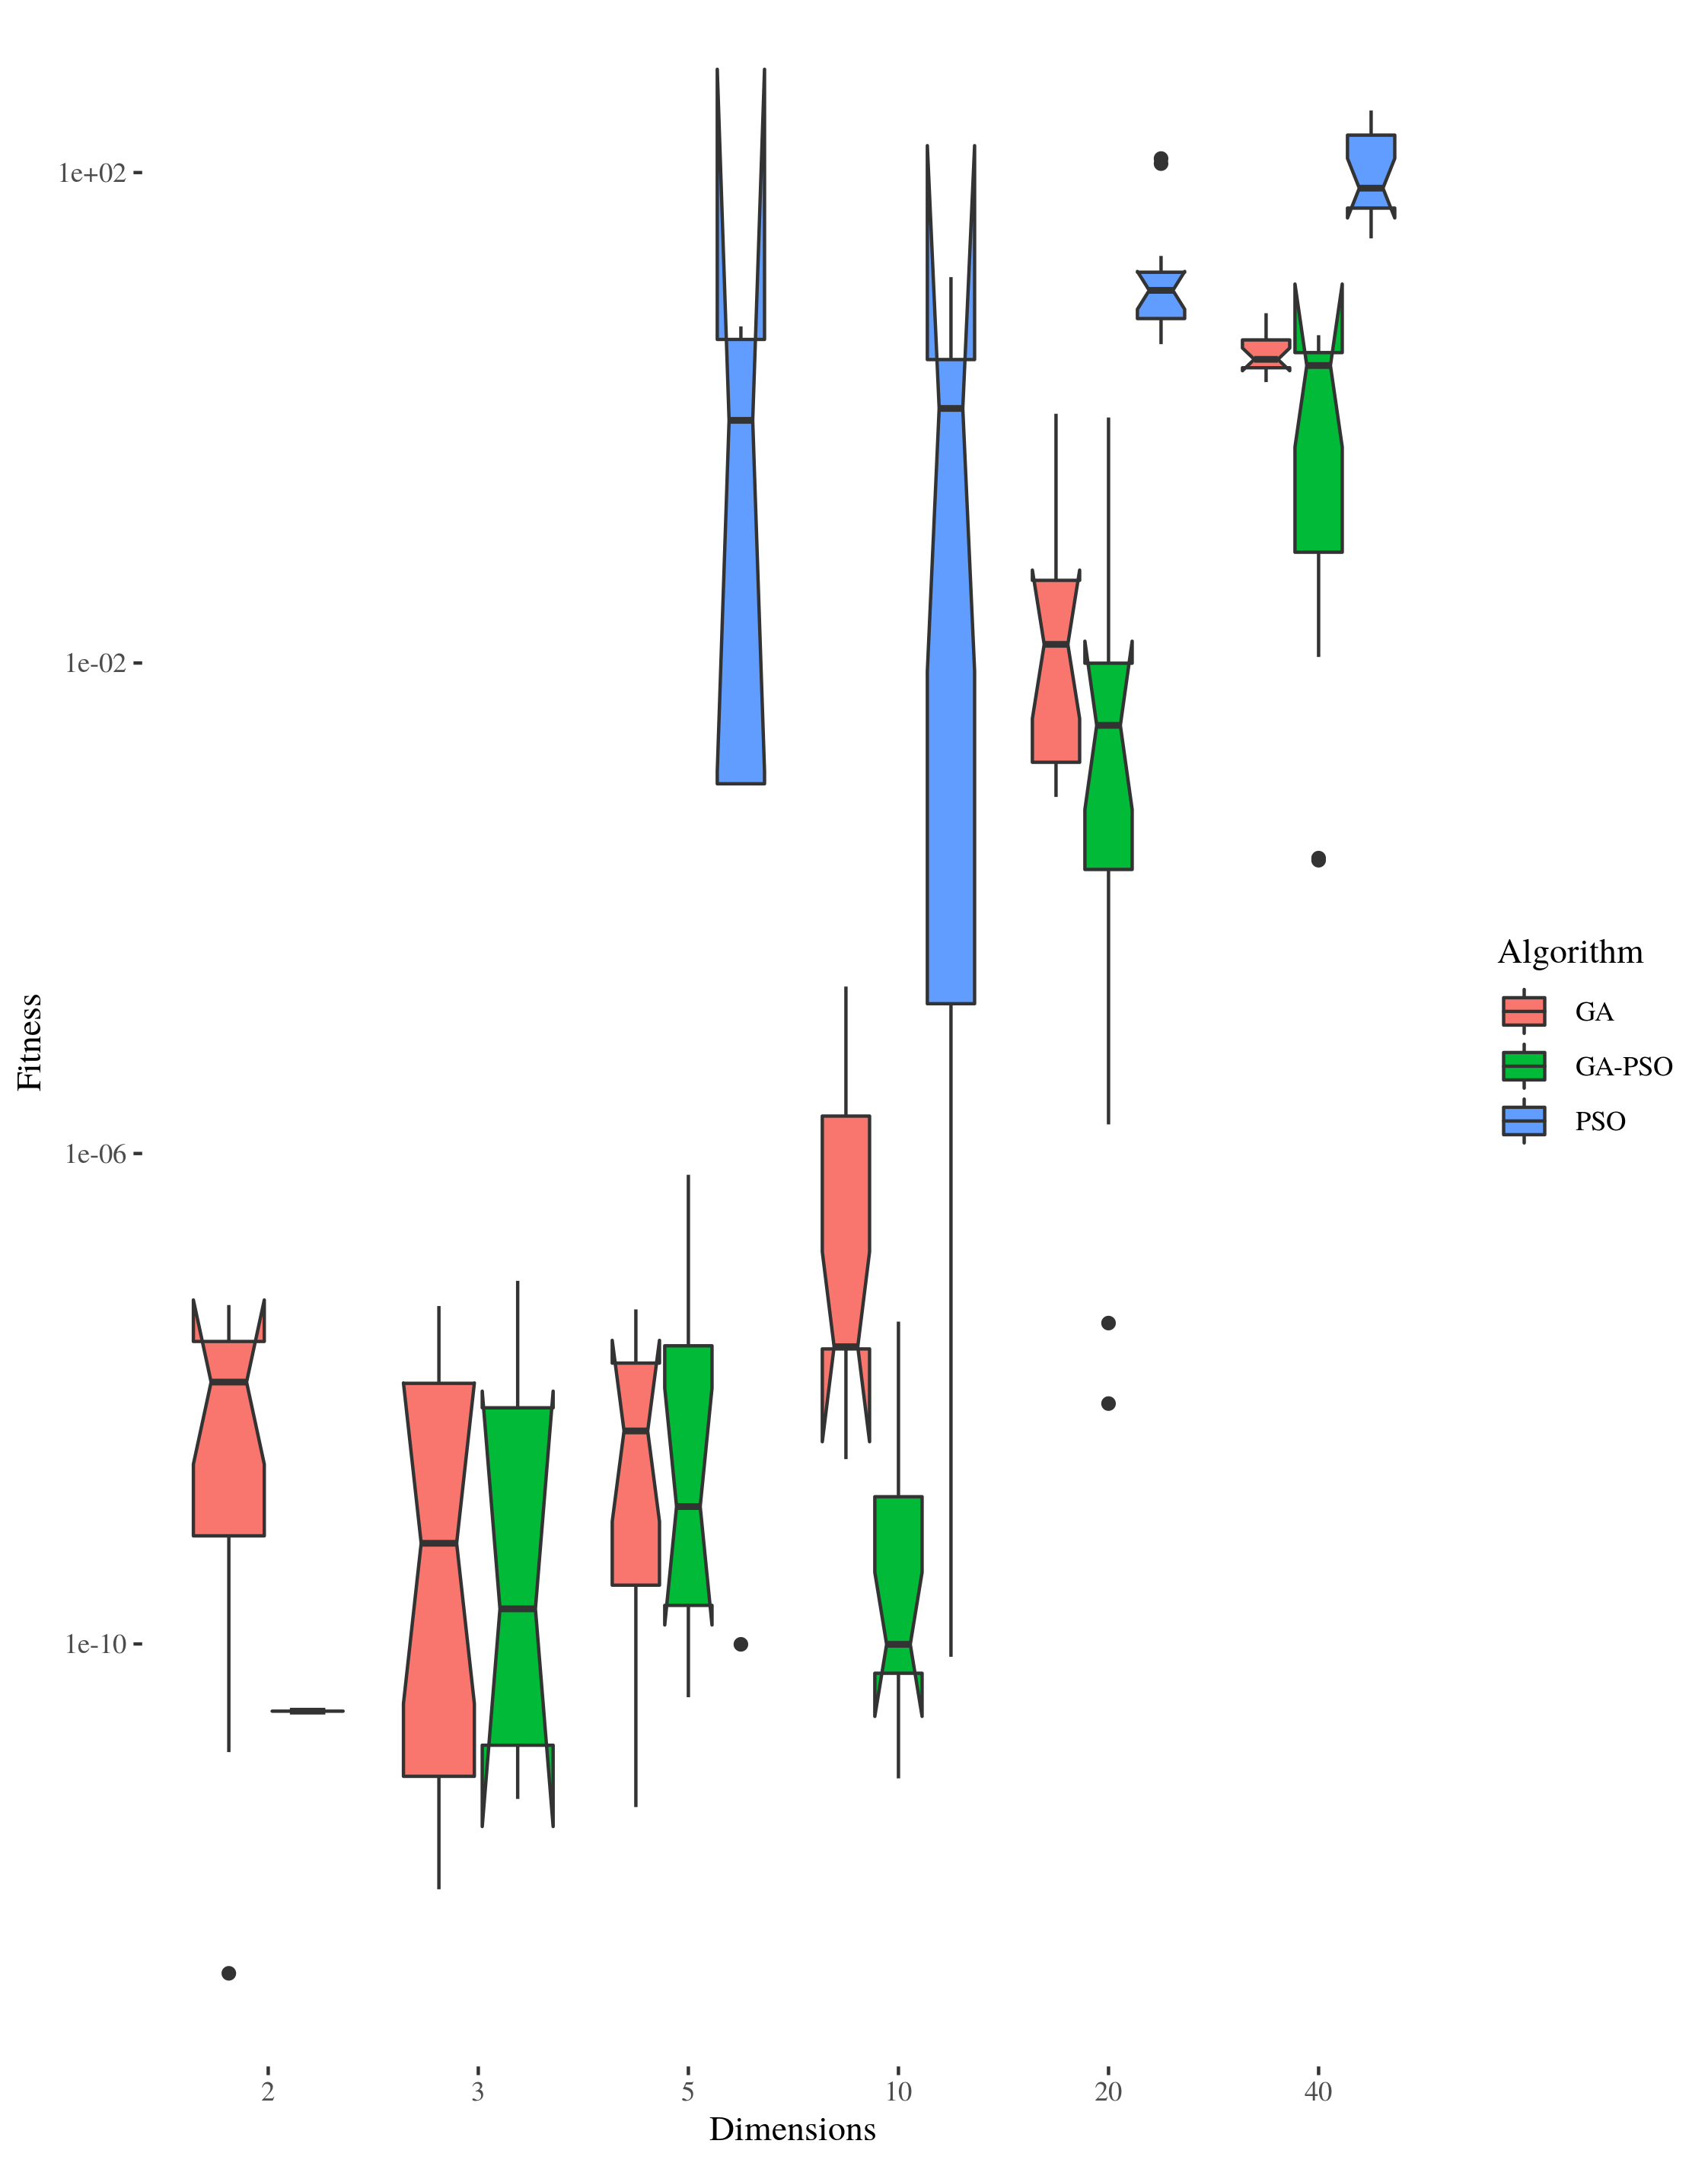
\includegraphics[width=0.32\linewidth]{img/rastrigin-boxplot.png}
                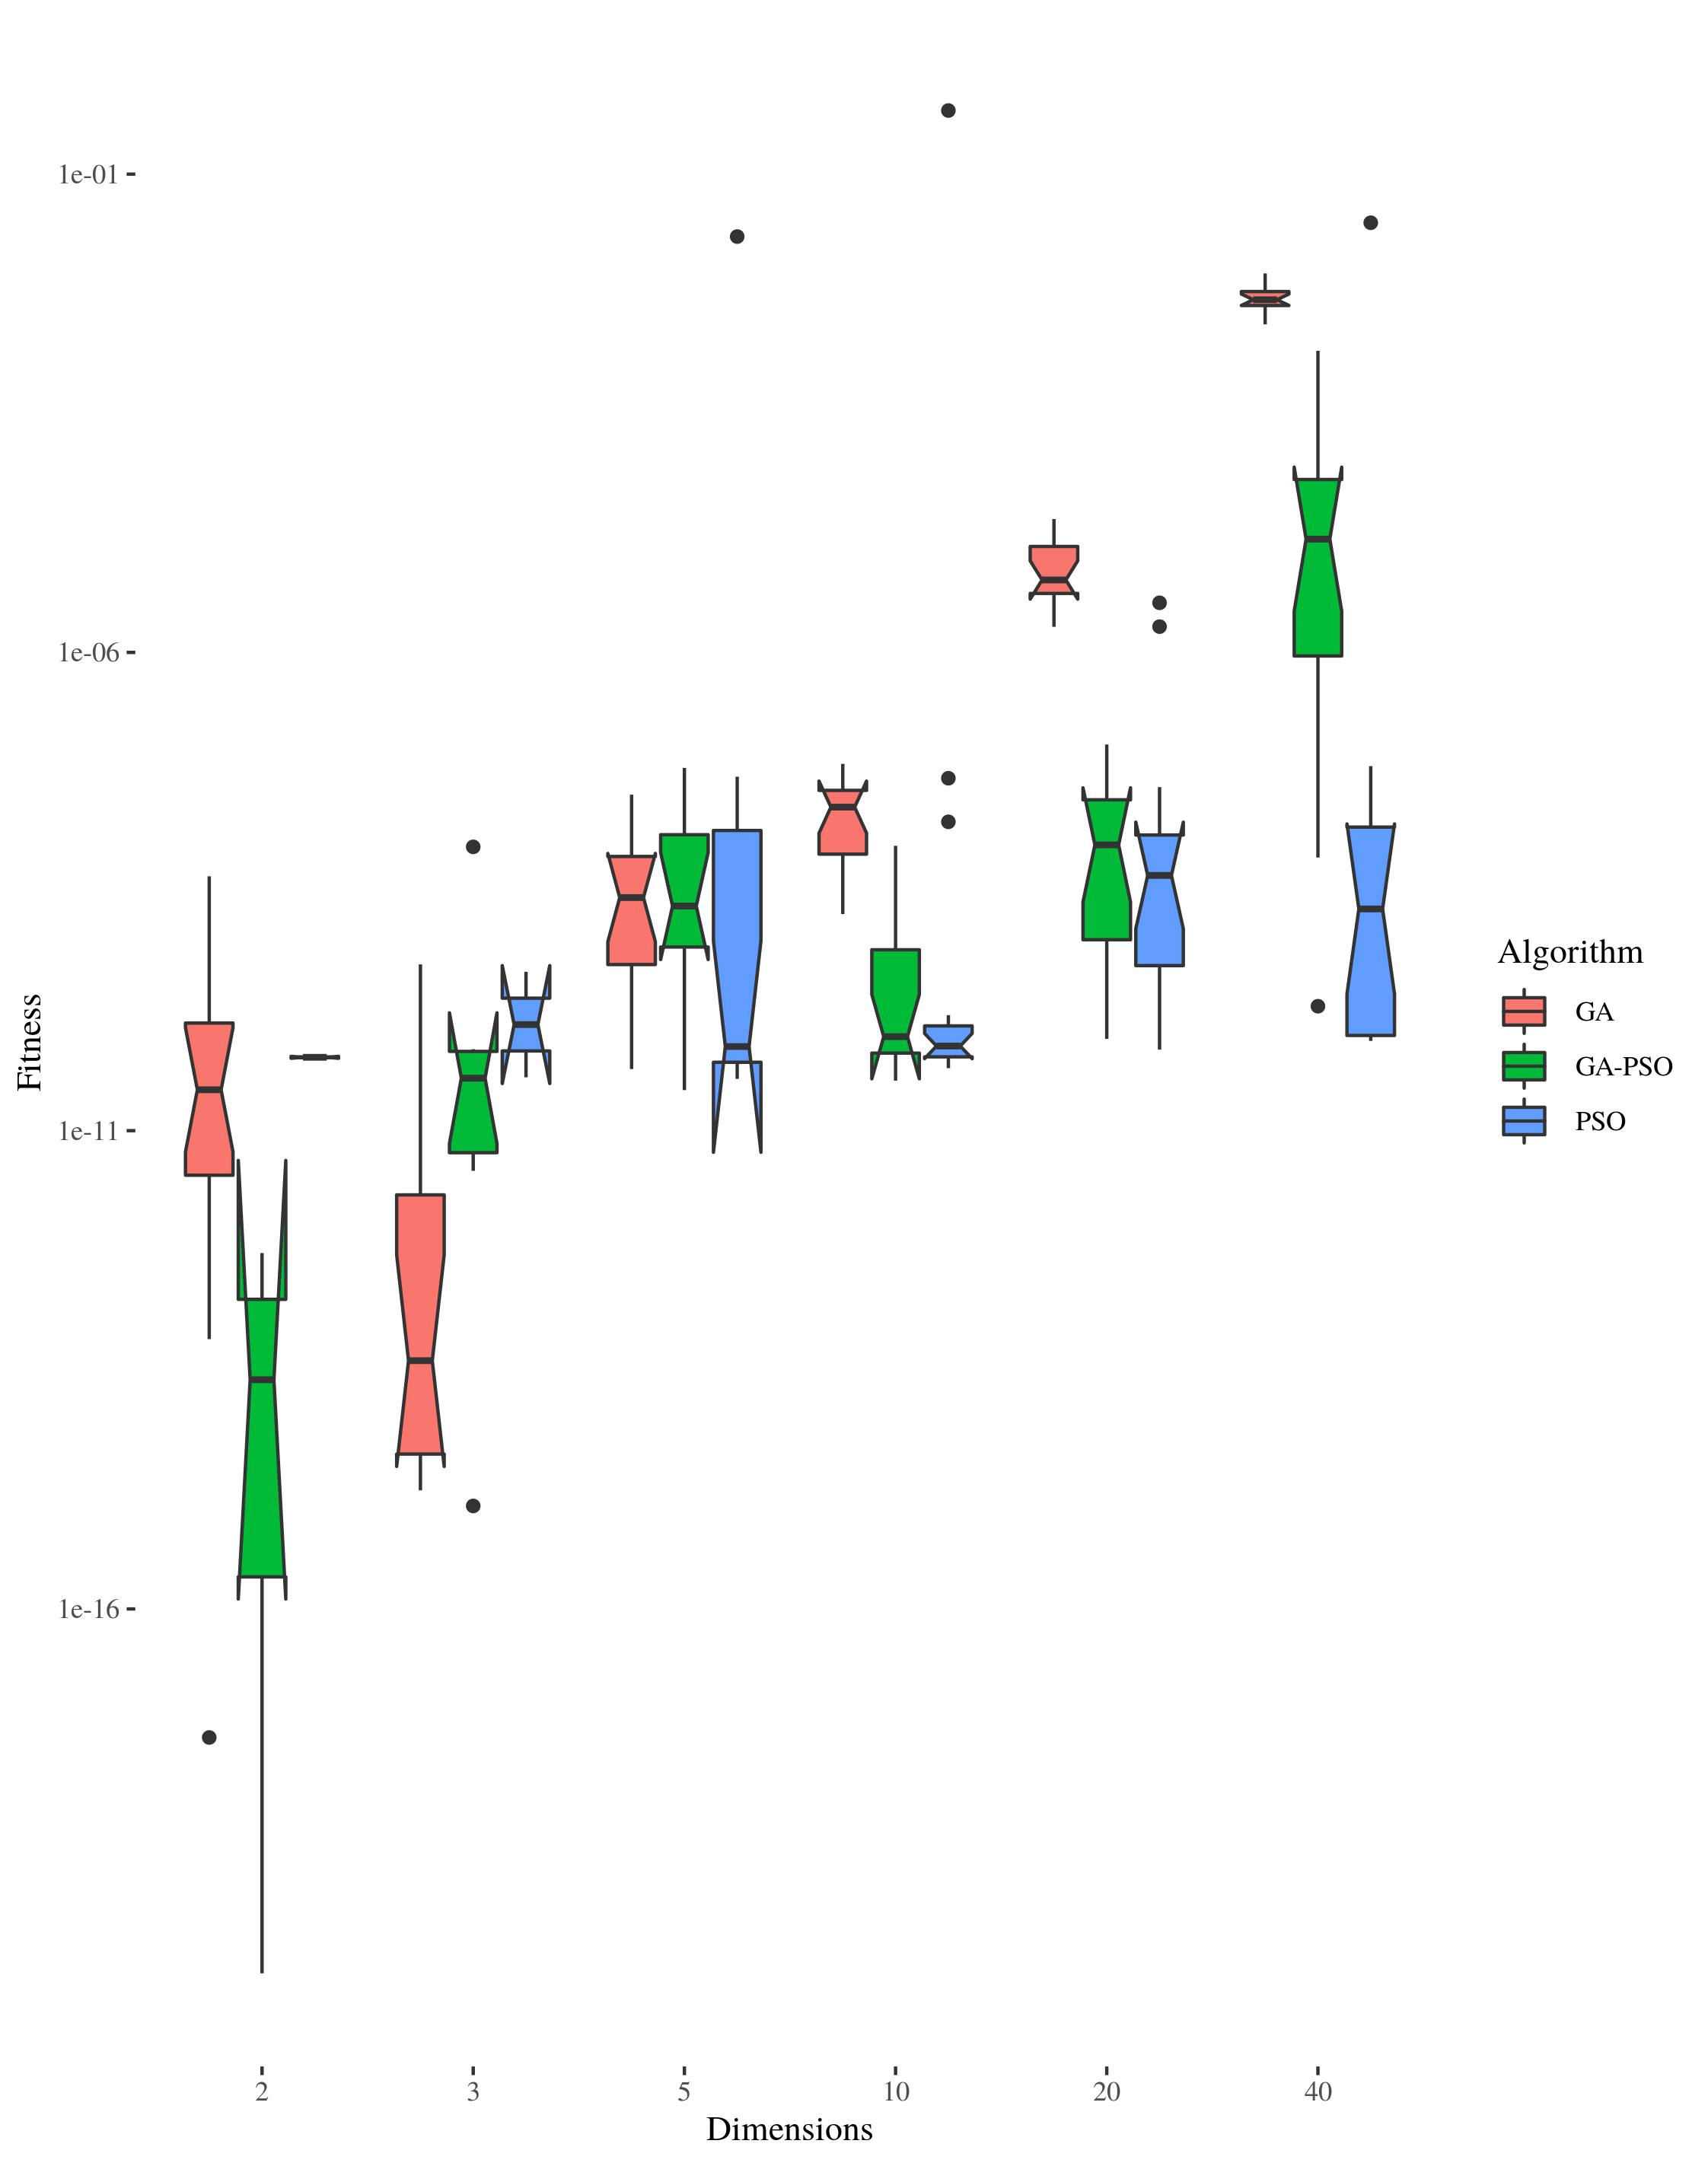
\includegraphics[width=0.32\linewidth]{img/sphere-boxplot.png}
                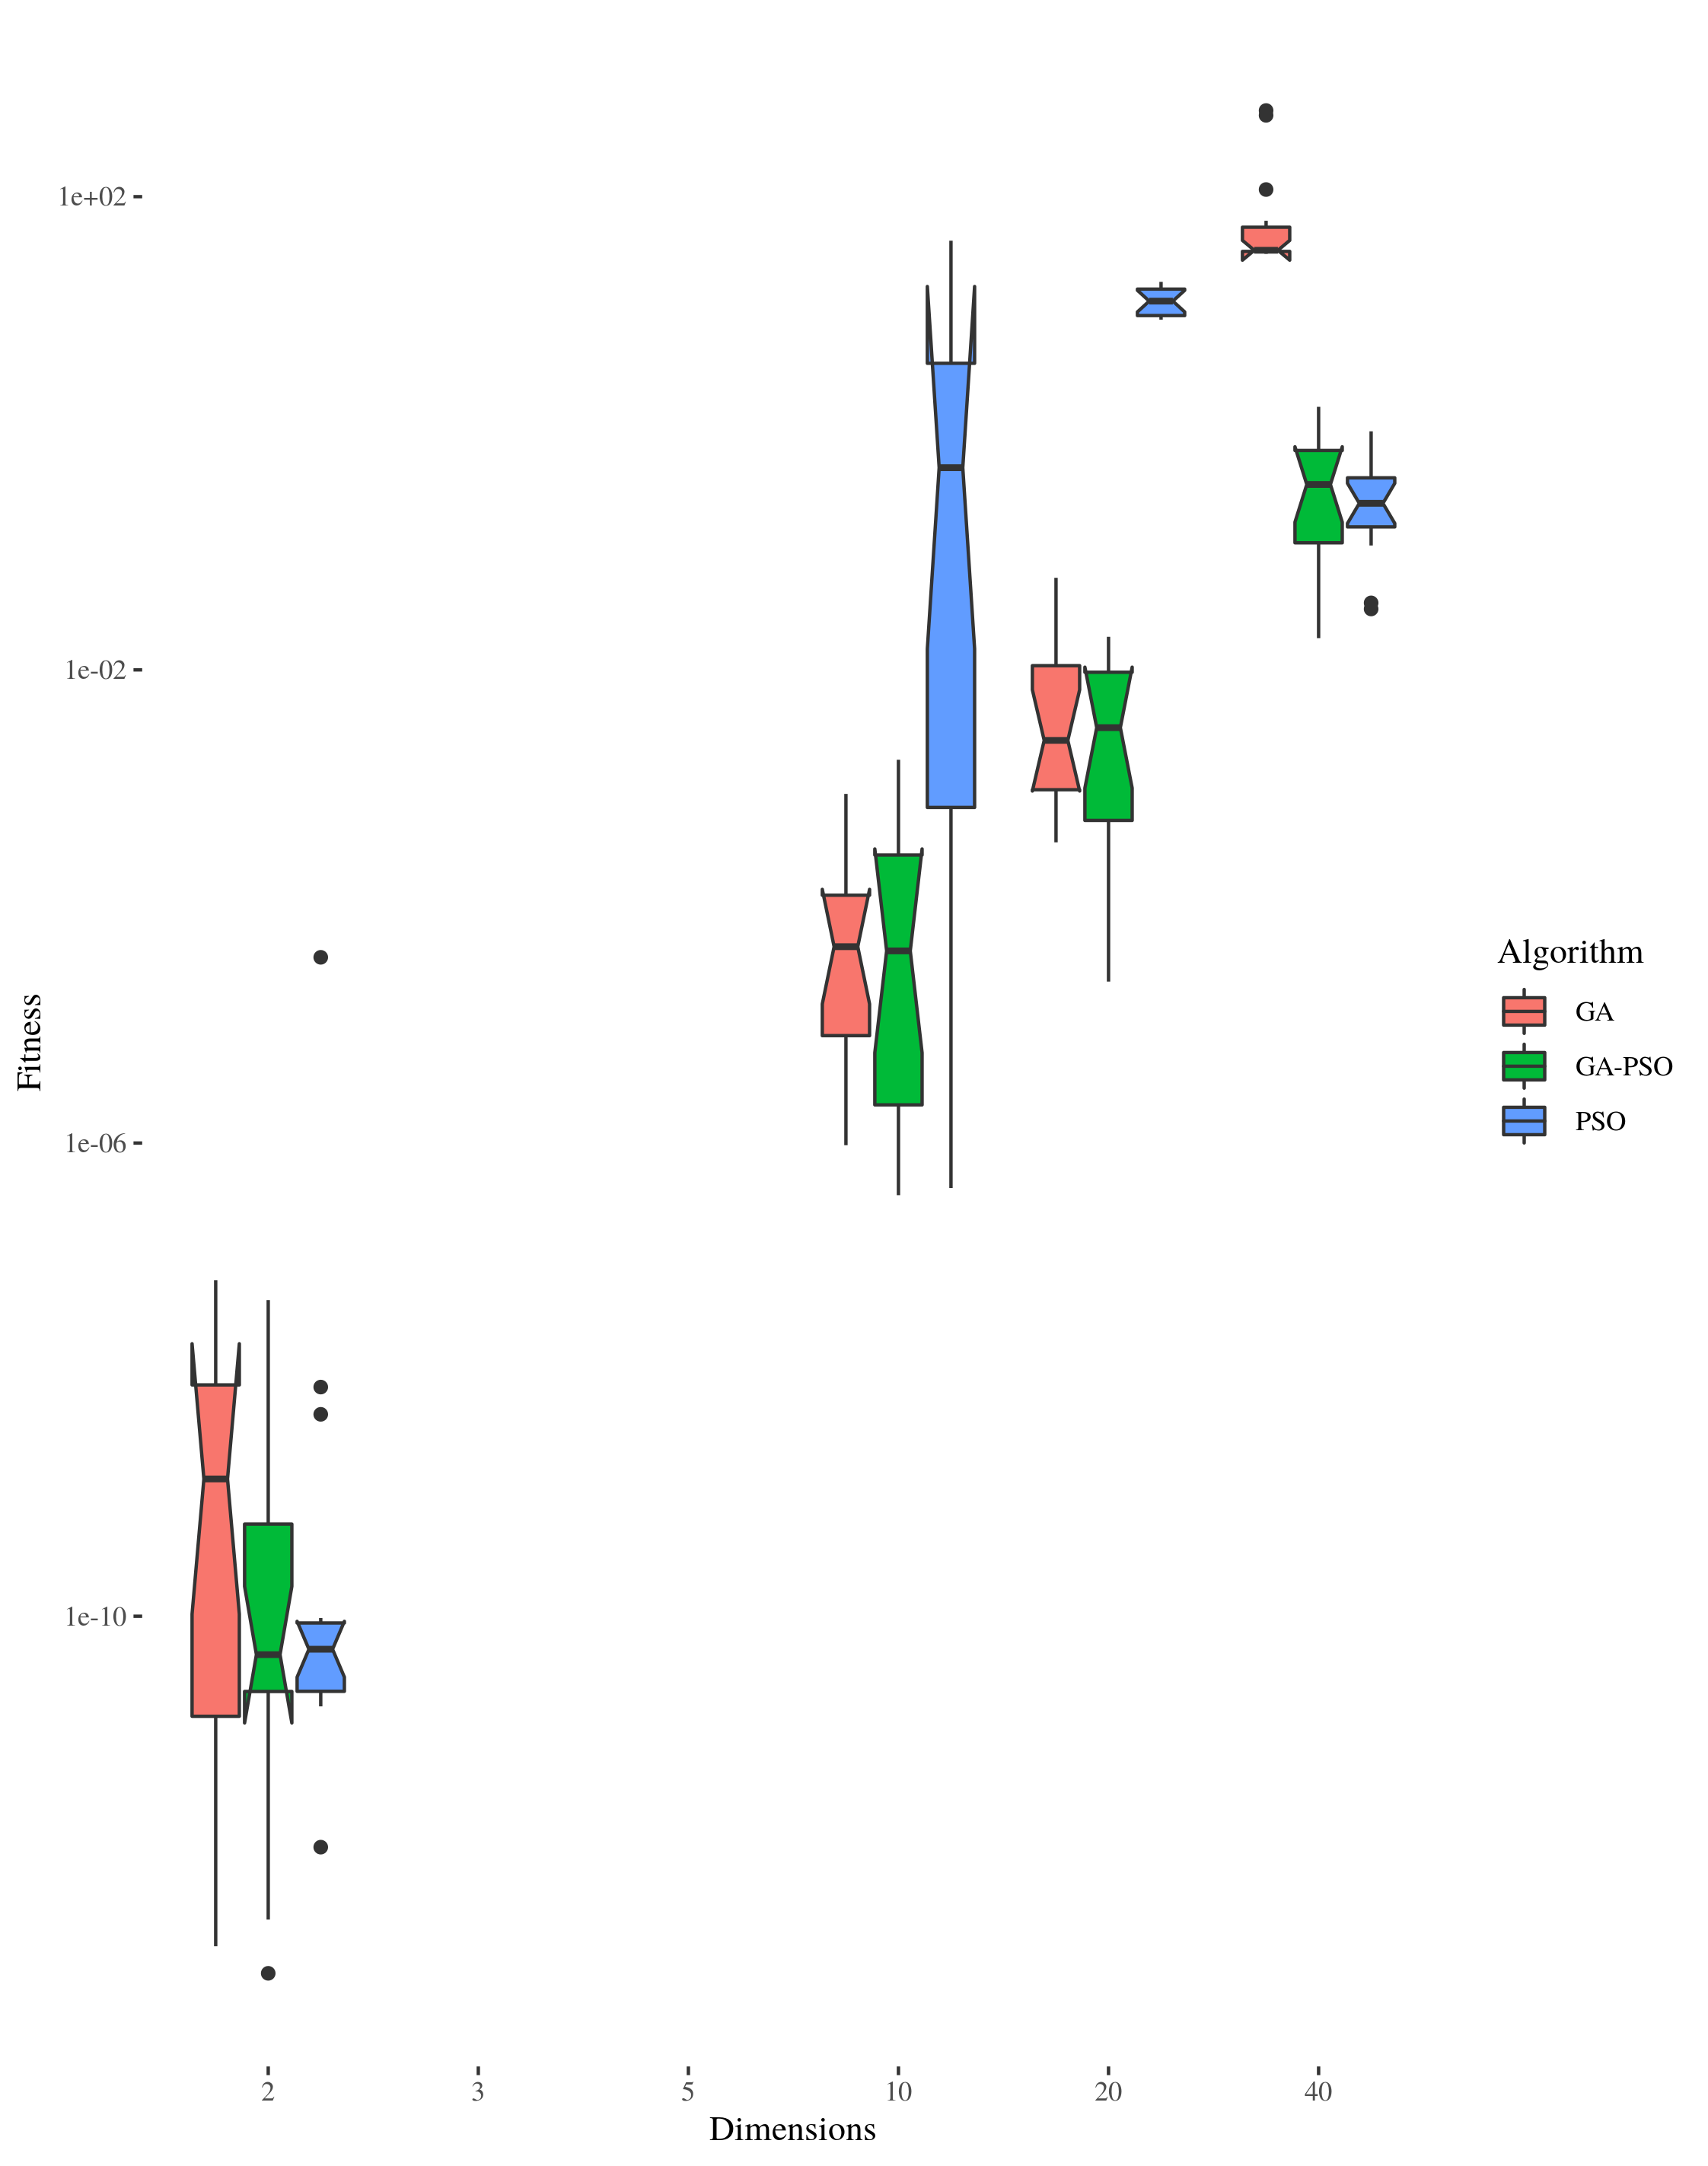
\includegraphics[width=0.32\linewidth]{img/rosenbrock-boxplot.png}
              \caption{Boxplot of results for, from left to right,
                Rastrigin, Sphere and Rosenbrock functions.\label{fig:boxplot}}
            \end{figure}
            
% ---- Bibliography ----
%
% BibTeX users should specify bibliography style 'splncs04'.
% References will then be sorted and formatted in the correct style.
%
% \bibliographystyle{splncs04}
% \bibliography{mybibliography}
%
\section{Conclusion}

This architecture is completely scalable and useful for implementation of
multiple algorithms, until now is only GA and PSO but according to the results
with this kind of architecture there is no limit and it works better than
cross-breed multi-population with only one algorithm, also every experiment executes in
short times because serverless functions searching in an asynchronous way
getting a fast convergence.

\section{Future work}

% Reference with interesting challenges: li2015multi 
% Dynamic optimization needs: a non-fixed number of populations, 
% how to increase (measure) diversity in dynamic optimization problems.
% restrict or not restrict populations in certain areas.

To get a continuous improvement it is believed that it is required a sort of
mutation applied to the sub-populations. This mutation would be a swapping type,
taking the algorithm parameters from the best and the worst sub-populations,
increasing the possibilities to get an optimal result, preventing get stuck into
a local optimum. Of course, it is expected to use this architecture using more
algorithms than GA and PSO.


\bibliography{samplepaper}
      \bibliographystyle{ieeetr}
  
\end{document}
